\chapter{Realtidsplanlægning}
\label{chap:rtp}
\fxnote{Kom ind på starvation et eller andet sted.}
Det andet anvendelsesområde vil vi behandle, med henblik på at inføre tid i \pycsp , er Real-time planlægning (RTP). Vi vil i dette kapitel gennemgå RTP samt diskutere hvordan det kan implementeres i \pycsp. 

RTP er baseret på den kendsgerning at nogle begivenheder i programmer kan være vigtigere at få udført end andre indenfor en afgrænset tidsperiode. Dette kan f.eks. være interrupts, input- eller output enheder eller interne processer. Med RTP tilknytter man en deadline for hver begivenhed, som bruges til at planlægge rækkefølgen for afvikling af begivenhederne. Formålet er at optimere antallet af begivenheder der når at blive udført inden deres deadline er overskredet. Normalt anses alle begivenheder for at være lige vigtige, og de planlægges ud fra en optimal udnyttelse af processoren. Denne optimale processorudnyttelse kan man være nødt til at gå på kompromis med hvis man ønsker at bruge RTP og derved prioritere visse begivenheder højere end andre. Man kan forestille sig en situation hvor man ikke starter en begivenhed med lav prioritet selv om den er klar, hvis man ved at en begivenhed med høj prioritet er klar kort tid efter, og venter derfor på at den er klar og igangsætter begivenheden med høj prioritet med det samme. 
RTP benyttes meget i specialiserede indlejrede systemer til f.eks medicinsk udstyr, kontrol af luftrummet, på rumstationen ISS\cite{Audsley1990} og mange andre steder. Det er dog også anvendeligt i mere gængse applikationer, typisk i forbindelse med en eller anden form for interaktion med den virkelige verden. 

I litteraturen omkring RTP bruges begreberne hard- og soft deadlines samt hard- og soft real-time systemer forskelligt, så vi vil i det følgende gennemgå hvordan vi definerer disse begreber. Vi har valgt at illustrere deadlines ved hjælp af time-value funktioner, hvor ``værdien'' indikerer det bidrag begivenheden bidrager med til systemets overordnede mål. 

\subsubsection{Kritisk deadline}
En kritisk deadline er en deadline som under alle omstændigheder skal overholdes for at opretholde systemets integritet. Såfremt en kritisk deadline overskrides vil der påføres skader på systemet som kan forårsage at systemets tilstand bliver udefineret. En kritisk deadline er illusteret på \cref{fig:hard-rtp}.

\begin{figure}
 \begin{center}
  
\includegraphics[scale=0.75]{images/critical-deadline}
	\caption{Begivenhed med kritisk deadline.}
	\label{fig:hard-rtp}
\end{center}
\end{figure}


\subsubsection{Hard deadline}
Vi definerer en begivenhed til at have en hard deadline såfremt en færdiggørelse af begivenheden efter deadlinen ikke tilfører systemet nogen positiv værdi. Modsat en kritisk deadline kan en overskridelse af en hard deadline accepteres. På \cref{fig:hard-dl} vises en hard deadline for en begivenhed. 

\begin{figure}
 \begin{center}
  
\includegraphics[scale=0.75]{images/hard-deadline}
	\caption{Begivenhed med hard deadline.}
	\label{fig:hard-dl}
\end{center}
\end{figure}

\subsubsection{Soft deadline}
Færdiggørelse af en begivenhed med en soft deadline, før dens deadline tilføjer den samme værdi til systemet som hvis den havde haft en hard deadline. Forskellen ligger i den tilførte værdi såfremt deadlinen overskrides. Hvor en hard deadline ikke tilføjer nogen værdi ved en overskridelse, vil en overskridelse af en soft deadline stadig tilføre en reduceret værdi ved færdiggørelse. Den tilførte værdi vil være omvendt proportional med længden af overskridelsen. \CRef{figure:soft-dl} illustrerer en soft deadline. 

\begin{figure}
 \begin{center}
  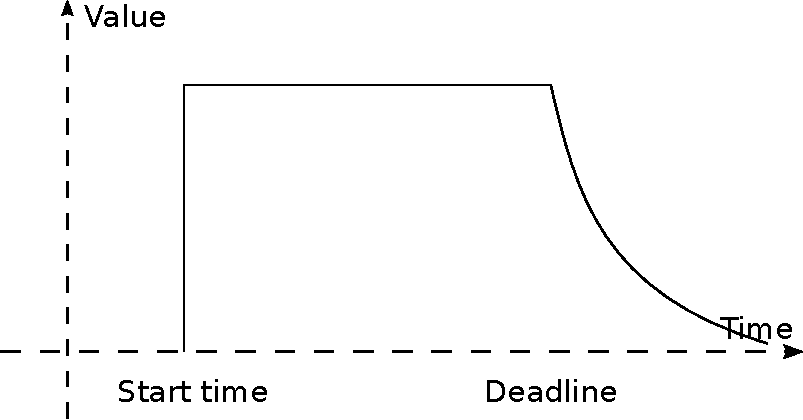
\includegraphics[scale=0.75]{images/soft-deadline}
	\caption{Begivenheden med soft deadline.}
	\label{figure:soft-dl}
\end{center}
\end{figure}

\subsubsection{Hard real-time system}
Et hard real-time system er defineret ved et system der har begivenheder med hard deadlines, og kan garantere at disse ikke overskrides. Ydermere skal systemet være derterministisk, så denne garanti kan gives på forhånd. Det giver ikke mening at snakke om kritiske deadlines i hard realtime systemer da de kun adskiller sig fra hard deadlines med henblik på konsekvensen af en overskreden deadline, hvilket per definition ikke må ske i et hard real-time system.  

\subsubsection{Soft real-time system}
Et soft real-time system kan indeholde alle typer deadlines men opstiller ikke nogen garantier for at de overholdes. Det vil typisk bruge en algoritme til at op- og nedprioritere hvilke deadlines der skal overholdes såfremt alle deadlines ikke kan overholdes.

Generelt vil der i et real-time system ikke være alle begivenheder der har den samme type af deadline. Nogle begivenheder har ingen deadline, nogle har en soft deadline, og få har en hard eller eventuelt en kritisk deadline. 
 
\section{Planlægning af begivenheder}
Planlægningen af hvilke begivenheder der skal køres hvornår, tager udgangspunkt i det overordnede formål med systemet. Generelt vil formålet være at minimere antallet af overskredne deadlines, men dette er sjældent det eneste kriterie der planlægges efter, ofte vil prioriteten for, og tiden det tager at udføre en begivenhed indgå i planlægningen. Eksempelvis vil man ofte prioritere at nå en kritisk deadline selv om det betyder at man overskrider to soft deadlines. 

%De fleste eksisterende real-time systemer arbejder på isolerede systemer, hvor planlæggeren har fuld kontrol over hele computeren. Derfor er hovedparten af forskningen indefor området gået til udarbejdelsen af specialiserede kerner og komplette operativsystemer\cite{damm1989real, jones1979staros, levi1989maruti,ramamritham14scheduling}. Vi ønsker i modsætning hertil ikke at udvikle en specialiseret kerne, men lade \sched en i \pycsp kunne planlægge processer efter bedste evne baseret på informationer den har om processerne.

For at foretage en planlægning af begivenheder der opfylder systemets formål bedst muligt, skal vi have så meget information om begivenheder som muligt - jo mere vi ved om dem jo bedre en planlægning kan der foretages. De relevante informationer i forhold til planlægningen er, hvornår en begivenhed forekommer, hvor lang tid den tager at udføre samt hvilken prioritet den har. 

Ud fra den tilgængelige viden kan der foretages en statisk eller dynamisk planlægning\cite{cheng1987scheduling}. Statisk RTP kræver at vi har alle de nævnte informationer om alle begivenheder. Herved kan vi på forhånd foretage en fuldstændig planlægning og allerede inden start have klarlagt om nogen deadlines vil blive overskredet. Såfremt vi ikke har alle informationer til rådighed, er vi nødsaget til at foretage en dynamisk planlægning. Dette vil ofte skyldes at vi enten ikke ved hvornår en begivenhed forekommer, eller at vi ikke har information om hvor lang tid der tager at udføre en begivenhed. I praksis vil det være svært at opstille eksakte værdier for hvor længe en begivenhed er om at blive udført og der benyttes derfor ofte estimater i stedet for. \fxnote{hvilken betydning har det at der benyttes estimater i stedet for eksakte værdier?}

%Overordnet kan begivenheder planlægges enten statisk eller dynamisk\cite{cheng1987scheduling}. I statisk RTP er alle begivenheder kendt på forhånd. Planlæggeren kan i dette tilfælde allerede inden start udregne om det er muligt at overholde alle deadlines. Alternativt planlægges begivenhederne dynamisk hvis der uregelmæssigt kan ankomme nye begivenheder der skal planlægges. 

%\fxnote{Motivationen her skal være at vi skal kende begivenheders frekvens og længde - skriv noget om det!}
%I realtidssystemer er næsten alle begivenheder cykliske, med enten en regelmæssig eller tilfældig frekvens. Begivenheder der forekommer med en regelmæssig frekevens kan være f.eks. være målinger der skal foretages med bestemte intervaller, hvor uregelmæssig frekvens ofte vil være tilfældet ved begivenheder der skal indtræffe som reaktion på udefrakommende input, f.eks. fejl eller alarmer. 

%\begin{shaded}
%Til planlægningen har planlæggeren behov for at vide hvor lang tid det vil tage at udføre en given begivenhed per periode, men da dette tal enten ikke er kendt eller fast for hver periode, bruges der ofte estimater. Dette medfører at en aperiodisk begivenhed kan ankomme på et vilkårligt tidspunkt og da planlæggeren kun har et estimat for tidsforbruget kan man  ikke tilknytte en ``hard deadline'' til aperiodiske begivenheder, da der altid findes en kæde af aperiodiske begivenheder der medfører en overskridelse af en deadline. 
%\end{shaded}

%\fxnote*{Dette skal måske flyttes eller omformuleres så vi ikke med det samme begrænses til dynamiske \sched}{I \pycsp kan der til alle tidspunkter tilføjes nye processer, og derfor vil vi kun beskæftige os med en dynamisk \sched. Desuden har man ikke med \pycsp fuld kontrol over hele operativsystemet. Mængden af processerkraft vi har til rådighed til kørsel af processerne vil derfor varriere uafhængigt af \pycsp, hvorfor vi heller ikke kan lave et pålidelig ``hard real-time system'', men fokusere på et ``soft real-time system''.}

\subsection{Metoder til skemaplanlægning}
Der findes adskillige metoder til at planlægge rækkefølgen af begivenheder. De adskiller sig fra hinanden med henblik på hvilke informationer der er til rådighed og hvad de optimerer efter. Vi har valgt at kigge på ``Rate monotonic algorithm''\cite{lehoczky1989rate,liu1973scheduling} og ``Earliest deadline first''\cite{liu1973scheduling} indenfor henholdsvis statisk og dynamisk skemaplanlægning.

Hvor processer isoleret set har behov for at udføre deres opgave inden deres deadline, har \sched en behov for kvantitativt at kunne organisere dem indbyrdes, således den til enhver tid kan vælge hvilken proces der skal udføres som den næste. Hovedformålet for en  \sched ~ er derfor at gå fra en række processer med tilknyttet deadline og eventuelt andre egenskaber til en prioriteret liste. \\
Der fokuseres i litteraturen på om en algoritme er stabil eller ej. Såfremt en algoritme er stabil vil man kunne definere en delmægnde af begivenheder, for hvilke man kan garanterer at de ikke overskrider deres deadline. 

\subsubsection{Rate monotonic algorithm (RM)}
RM er en statisk \sched, der fra start af udregner en prioriteret liste på baggrund af frekvensen af processens periode, dermed vil processer der oftet skal have udført deres periode en højere prioritet, end processer med lav frekvens. RM er todelt og i første del udføres før selve simuleringen udregnes  prioriteten for processerne, og udvælger hvilke processer der kan medtages i selve udførslen. Anden del står for udvælgelsen af processer  under simuleringen, og her vælges simpelt den proces med den højeste prioritet. 

Et problem for RM er at ved udvælgelsen af processer der kan medtages har man ikke en optimal udnyttelsen af processorkraft. \Citeauthor{lehoczky1989rate} er kommet frem til at ``worst-case'' er udnyttelsen i gennemsnit 88\\cite{lehoczky1989rate}. Et større problem i relation til implementering i \pycsp er dog at RM er dog at den er statisk. Til gengæld er algoritmen stabil ved en overskridelse af deadline for en proces. 

\subsubsection{Earliest deadline first (EDF)}
Som alternativ til den statiske \sched, hvor man ikke kan ændre prioriten af processen løbende gennem simuleringe, findes de dynamiske \sched er, hvor er EDF er et eksempel. Her evalueres prioriterne af processerne dynamisk igennem simuleringen og evaluere dermed løbende hvilke processer der skal udvælges. I EDF har den proces hvis deadline ligger tættest på højest prioritet og den hvis proces har længst til deadline den laveste prioritet. Aperiodiske processer kan i EDF indgå på lige fod med de periodiske da man til hvert processkift evaluere hvilken der har den nærmeste deadline, som både kan være en periodisk proces som en aperiodisk.

Udnyttelsen af processorkraft kan i EDF komme op på 100\, da alle processer bliver planlagt løbende i modsætning til RM der foretager et valg om en given proces kan planlægges.  Ulempen ved EDF er den ikke er stabil i det vi ikke har kontrol over hvilke processers deadline der bliver overskredet. Dette er specielt et problem hvis man har en en uhomogen samling processer hvor en mindre del er kritiske.

\subsubsection{Least Laxity(LL)}
LL er en modifikation af EDF. LL kigger på hvor lang tid en begivenhed tager at udføre sammenholdt med hvor lang tid der er til deadline for begivenheden. Laxity er defineret som deadline minus tiden det tager at udføre begivenheden. Laxity bliver altså et udtryk for hvor presserende det er at igangsætte en begivenhed for at den kan nå sin deadline. I LL bruges dette til at prioritere de begivenheder der har mindst laxity højest når begivenhederne planlægges. \\
\\
I systemer hvor begivenheder ikke er isolerede men kan have interne afhængigheder, kan der opstå det problem der hedder prioritetsinvertering\cite{sha1990priority}. Dette problem opstår hvis en begivenhed med høj prioritet er afhængig af en begivenhed med en lavere prioritet. Derved bliver begivenheden i praksis kørt med den lavere prioritet da den ikke er klar før begivenheden med lav prioritet er færdig. Problemstillingen kan vises klart med følgende eksempel. Forestil dig tre begivenheder ($B_0,B_1,B_2$)med prioriteterne $Pr_0>Pr_1>Pr_2$. Først udvælges $B_0$ da denne har højst prioritet, men stopper da den er afhængig af kommunikation fra $B_2$. Den næste begivenhed der udvælges vil være $B_1$, og dermed bliver $B_0$ unødigt forsinket mens $B_1$ kører.\\
En ofte benyttet metode til at undgå priotetsinvertering er priotetsnedarvning. Ved at benytte denne løsning vil en begivenhed med lav prioritet, som en begivenhed med høj prioritet er afhængig af, nedarve prioriteten fra den begivenhed der venter på den. Herved sikres det at begivenheder med høj prioritet ikke kommer til at vente unødigt på prioriteter med lav prioritet. \fxnote{flere løsninger på prioritetsinvertering bør nok nævnes.}


\section{Realtime planlægning i \pycsp}
\label{sec:rtp-pycsp}
\fxnote{(Flyttet fra RTP overordnet) Husk at snakke om begrænsning af greenlets mht. parallelitet når vi arbejder i realtid}
Da vi ønsker at introducere RTP i \pycsp, er der er række forhold, som vi skal tage højde for. Vi vil i dette afsnit tage udgangspunkt i de ovenstående opstillede muligheder og sammenholde dem med \pycsp. 

I \pycsp kan vi anskue processerne som begivenheder og derved bruge skemaplanlæggeren i \code{greenlets}-versionen til at styre hvilken proces og dermed hvilken begivenhed, der udføres. Vi har ikke umiddelbart informationer om, hvor lang tid en proces er om at blive udført, og det vil kræve en analyse af den enkelte proces at udlede estimater for det. Vi har valgt at fokusere på selve planlægningen af processerne og ikke på analysen. Dermed har vi ikke mulighed for at benytte RM og LL algoritmerne, da de begge benytter information om udførselstiden for en proces. Derved har vi EDF tilbage som mulighed, hvilket vi i det følgende vil implementere. En udvidelse af \pycsp til at benytte EDF er forholdsvis ligetil. Der skal laves en mulighed for, at brugeren kan angive en deadline til en proces, og vi skal ved kontekstskift sikre, at vi aktiverer den proces, der har den førstkomne deadline. Såfremt en deadline overskrides, skal vi have funktionalitet, til at håndtere dette. 

\pycsp har per definition interne afhængigheder mellem processerne i form af kommunikation over kanaler, og vi kan derfor opleve problemer med prioritetsinvertering. Den eneste metode til håndtering af dette, der kan bruges sammen med \pycsp, er prioritetsnedarvning, da de andre metoder forudsætter prioritetsinverteringen  sker som resultat af tilgang til kritiske regioner og ikke pga. kommunikation. Vi skal derfor også implementere prioritetsnedarvning for at sikre os mod prioritetsinvertering. 

Da vi benytter os af \code{greenlets}-versionen af \pycsp arbejder vi med en skemaplanlægger, der ikke kan foretage preemptive kontekstskift. Dette kan lede til problemstillinger som det er illustreret på \cref{fig:edf-nonpreemptive}. En metode til at mindske denne type problemer er at lade de enkelte processer afgive kontrollen med jævne mellemrum. Herved vil der blive foretaget en ny evaluering om hvilken proces, der skal aktiveres, og hvis der er processer, der har en nærmere deadline, som er blevet klar, aktiveres en af disse. Dette beror helt og holdent på at hver enkelt proces frivilligt afgiver kontrollen og gør det med jævne mellemrum, når den er aktiv. Dette betyder, at det er overladt til udvikleren at indsætte det på relevante steder i processens kode. 

\subsection{Tilknytning og overskridelse af deadlines}
Som udgangspunkt skal vi kunne håndtere, at en proces kan have forskellige typer deadlines. Umiddelbart er det oplagt, at der for hver proces tilknyttes en deadline samt hvilken type, det er. Dette giver mulighed for, at vi kan differentiere i den måde vi håndterer en overskreden deadline. F.eks. kan vi stoppe systemet helt i tilfælde af overskridelse af en kritisk deadline, kaste en exception ved en hard deadline og blot registrere overskridelser af soft deadlines. Uanset hvilken handling vi vælger at tilknytte til de respektive overskridelser, vil der altid være situationer, hvor den valgte handling ikke er optimal. 

Vi har derfor valgt en anden løsning, hvor en proces blot kaster en exception, hvis den overskrider en deadline. Dette overflødiggør, at der tilknyttes en specifik type deadline til en proces, da håndteringen af den kastede exception overgives til udvikleren. Det er herved op til den enkelte udvikler at definere, hvad der skal ske i hver enkelt proces, såfremt den overskrider en deadline. Dette giver den største frihed til at tilpasse håndteringen til den enkelte proces og applikation. 

\subsection{Udvælgelse af proces}
Udvælgelsen af hvilken proces der skal aktiveres, ved et kontekstskift, er givet ud fra vores valg af EDF. Som beskrevet i \cref{sec:edf} specificerer EDF, at det altid processen med den nærmeste deadline der skal aktiveres. For at opnå dette kan vi benytte stort set samme metode som vi brugte i \des. I \des sorterede vi processerne efter hvilket tidskridt de skulle aktiveres i, her kan vi sortere dem ud fra deres deadline.  

\subsection{Kanalkommunikation}\label{sec:rtp-kommunikation}
I litteraturen for  RTP fokuseres der kun på udvælgelsen og planlægningen af processer i \sched en. I \pycsp er kommunikation blokerende, hvilket betyder at fra en proces, ønsker at kommunikere, er den blokeret, indtil kommunikationen er gennemført. Ved one-to-one kanaler, er der kun en proces i hver ende, og derfor er  processen garanteret at gennemføre kommunikationen når modparten er klar til at kommunikere. Har processerne forskellige prioriteter risikere man prioritetsinvertering, og kan afhjælpe det med prioritetsnedarvning. 

I \pycsp er one-to-one kanalerne blevet fjernet, og erstattet af any-to-any kanaler, der ud fra et teknisk synspunkt er mere generelle og kan alt som one-to-one kanalerne kan. I any-to-any kanalerne er man ikke begrænset til kun at have en proces i hver ende af kanalen, men der kan være et vilkårligt antal processer. 
Benyttes prioritetsnedarvning på any-to-any kanaler, er man ikke som ved one-to-one kanaler sikret at det  processen der startede  prioritetsnedarvningen der får gavn af den, da parringen mellem processer der ønsker at kommunikere i \pycsp tilfældigt. Når processer kommunikere i  any-to-any kanaler kan man derfor med fordel sikre at det altid foregår mellem de to processer der har den højeste prioritet.


\subsection{Prioritetsnedarvning}\label{sec:rtp-pycsp-nedarvning}
At introducere prioritetsnedarvning i \pycsp virker umiddelbart ligetil, idet vi kan se de indbyrdes afhængigheder klart ud fra forbindelserne gennem kanalerne. Der kan forekomme andre afhængigheder, som er mindre synlige, men vi mener ikke disse vil forekomme i velskrevne CSP applikationer, og vi har derfor valgt at begrænse os til afhængigheder repræsenteret vha. kanaler. På trods af den umiddelbare simplicitet skal vi overveje hvornår, hvem og hvor længe, der skal arves i forbindelse med prioritetsnedarvning.

\subsubsection{Ændring af prioritet}
\label{sec:aendring-af-prioritet}
Vi arbejder med et dynamisk system af processer, hvor en proces, på baggrund af sin tilstand, er afhængig af forskellige andre processer for at kunne arbejde videre. 
Hvis vi højner prioriteten på alle processer, der er forbundet til en proces med høj prioritet, vil mange af processerne, der arver den høje prioritet, reelt ikke kunne bidrage til udførelsen af den proces, der starter med høj prioritet. Det er en bedre løsning, at det kun er den eller de processer, der kan sikre videre udførsel af den aktuelle proces, der tildeles højere prioritet. Hvis eksempelvis en proces med høj prioritet ønsker at skrive på en kanal, skal alle processer, der læser på den kanal, arve den høje prioritet, men de processer, som ønsker at skrive til en anden kanal, som processen med høj prioritet læser fra, skal ikke arve den høje prioritet. Generelt set betyder det, at der kun skal udføres prioritetsnedarvning, såfremt en højt prioriteret proces venter på at kommunikere, uden der er andre processer, der er klar til at indgå i den ønskede kommunikation. 

Vi har nu begrænset os til, at det kun er de processer der kan indgå i kommunikation over en kanal, der arver en prioritet. Med any-to-any kanaler findes der dog et vilkårligt antal processer i hver kanalende, og man risikerer en prioritetsdevaluering ved at lade flere processer arve en høj prioritet. I klassisk \csp findes der modsat hertil one-to-one kanaler, hvor man er sikret at det kun én proces' prioritet der bliver højnet ved prioritetsnedarvning. Forskellen kan illustreres af \autoref{fig:one-to-one-inheritance} og \cref{fig:any-to-any-inheritance}\fxwarning{tjek sidenr. er korrekt for de to figurer inden aflevering}. På \autoref{fig:one-to-one-inheritance}, bliver en proces' prioritet hævet fra fem til 10. Modtageren kan uden afbrydelser arbejde hen mod at kunne kommunikere, da afsenderen venter. I \autoref{fig:any-to-any-inheritance} bliver alle tre processers prioritet hævet til 10 og de vil skulle kæmpe mod hinanden for komme frem til en tilstand hvor de ønsker at kommunikere. 

\begin{figure}
 \begin{center}
  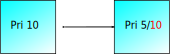
\includegraphics[scale=1.00]{images/one-to-one-inheritance}
\caption{Procesnetværk med en afsender og en modtager. Afsenderen har prioritet 10, mens modtageren har en initiel prioritet på fem. Modtageren  får via prioritetsnedarvning hævet sin prioritet til 10. (Højere er bedre)}
  \label{fig:one-to-one-inheritance}
  \end{center}
\end{figure}

\begin{figure}
 \begin{center}
  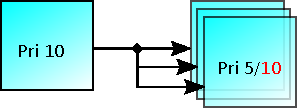
\includegraphics[scale=1.00]{images/any-to-any-inheritance}
  \caption{I dette eksempel findes der tre modtagere, som alle får hævet deres prioritet til 10.}
  \label{fig:any-to-any-inheritance}
  \end{center}
\end{figure}

Prioritetsnedarvning i et miljø med any-to-any kanaler har dermed en risiko for at medføre prioritetsdevaluering. Man kan forstille sig forskellige metoder til at eliminere eller minimere problemet f.eks ved at begrænse antallet af processer, der kan modtage en prioritetsnedarvning. Dette kunne gøres ved kun at lade en enkelt proces arve prioriteten,  men så skal man tage stilling til, hvilken proces, der skal udvælges. Dette kunne være den proces, der er tættest på at indgå i kommunikationen.  Udvælgelsen af processer må dog bero på en analyse af den enkelte applikation og dens aktuelle tilstand. Da vi ikke ønsker at begynde på en analyse af brugerens kode, må vi nødvendigvis sende prioritetsnedarvningen til alle processerne på kanalen. For at løse problemet vil vi i stedet fokusere på at minimere antallet af processer, der starter prioritetsnedarvningen, og det tidsrum processerne har arvet en prioritet.

Når kommunikationen på kanalen er gennemført, befinder processens sig i en anden tilstand og er afhængig af noget andet for at komme videre i sin udførsel. 
Når det midlertidige afhængighedsforhold ophører skal processer der har arvet en prioritet miste denne. Der skal selvfølgelig tages højde for at en proces kan arve forskellige prioriteter fra forskellige andre processer, så det skal være muligt at falde tilbage til den næsthøjeste arvede prioritet, i stedet for blot at skifte tilbage til den oprindelige prioritet. 

\subsection{Alternation}
Det er dog ikke kun i forbindelse med almindelig kommunikation vi skal forholde os til introduktionen af processer med et prioritet. I kodestrukturen \code{alternation}
 har en udvikler mulighed for at foretage et  prioriteret valg mellem flere forskellige kanaler. Et prioriteret valg mellem flere kanaler, kan dog være i konflikt med de processer som får opfyldt deres kommunikation. 
  
\citeauthor{Burns1990} beskriver og illustrerer præcist denne problemstilling i \citetitle{Burns1990}\cite{Burns1990}. Til at illustrere problemet beskriver de et eksempel, som er vist i \cref{lst:pri-select}. Denne kodestump viser et prioriteret valg mellem kanalerne A1 og A2. Til hver kanal er tilknyttet en proces, P1 og P2. Disse to processer har en prioritet tilknyttet på hhv.  Pri1 og Pri2. \CRef{tab:prioritizedSelect} viser hvilken kanal der bliver valgt, afhængig af processernes prioritet.

\begin{lstlisting}[firstnumber=1 ,float=hbtp, label=lst:pri-select, caption={(priority) select. Eksemplet er kopieret fra \cite{Burns1990}}]
(priority) select
   A1 -- Process P1
 or
   A2 -- Process P2
 end select
\end{lstlisting}

\begin{table}[htbp]
	\centering
	\begin{tabular}{lccc}
       	\toprule
                        & Pri1 > Pri2 & Pri1 = Pri2 & Pri1 < Pri2\\
        \midrule
	    priority select & A1          & A1          & ?  \\
        \bottomrule
        \end{tabular}
    \caption[]{Konflikten ved brug af prioriteret valg og procesprioriteter. Eksemplet er kopieret fra \cite[160]{Burns1990}}\\
    \label{tab:prioritizedSelect}
\end{table}

Man kan af \cref{tab:prioritizedSelect}  konstatere at der opstår en konflikt i kolonne tre, hvis udvikleren foretrækker en kanal, hvor den  tilknyttede proces' prioritet er lavere  end den anden proces'  prioritet. Man vil ikke kunne opfylde begge krav om både at kommunikere med den proces med højst prioritet, og lade udvikleren bestemme kanalen. For \citeauthor{Burns1990} er løsningen en ``orthogonal solutions'', der håndterer begge typer prioriteter. De ønsker overordnet set to typer udvælgelsesmetoder, weak- og strong Select. Weak select sorterer primært efter processernes prioritet og sekundært efter det prioriterede valg. Strong select udvælger udelukkende processer efter det prioriterede valg. De forstiller sig, at weak select skal bruges som den primære metode, men i specielle tilfælde skal en udvikler have mulighed for at tvinge et prioriteret valg igennem.

I artiklen fra \citeauthor{Burns1990} har de kun beskæftiget sig med one-to-one kanaler, og det er denne antagelse der medfører at et valg af kanal medfører et valg af en proces og dennes prioritet. Dette er ikke en mulighed i \pycsp hvor kanalerne er af typen any-to-any. Et valg af en kanal, medfører derfor ikke en direkte kobling til en proces, men til vilkårligt mange processer, der kan have individuelle  prioriteter. I \cref{sec:rtp-kommunikation} kommer vi frem til at kommunikationen altid skal sørge for at det er den højst prioriterede proces der kommunikerer. Dette kan bruges i \code{alternation} til at finde den højeste prioritet blandt de processer der er klar til at kommunikere, og bruge denne prioritet til udvælgelsen af kanal i \code{alternation}.

På baggrund af artiklen har vi valgt at \code{alternations} udfører en weak select, da denne version egner sig bedst til RTP . Vi vil i vores version ikke inkludere en strong select. Dette gør vi ud fra en betragtning om at den kun bør bruges i sjældne tilfælde,  da den vil modarbejde ideen bag RTP. Hvis en udvikler alligevel ønsker denne funktionalitet, vil har godt kunne opnå det i \pycsp, men vi ønsker ikke at tilskynde brugen, ved direkte at inkludere den.

\phantomsection
\label{misc:kanal-prioritet}
\subsubsection*{Prioritetsnedarvning i \code{alternations}}
Vi har som nævnt en klar kæde af afhængigheder i \pycsp men vi skal være opmærksomme på ikke at højne processers prioritet unødigt. Dette kan let blive tilfældet såfremt vi ikke holder ordentligt styr på, hvorfor en proces har den prioritet, den har, om den er sat af udvikleren, eller den er nedarvet. Man kan forestille sig en situation, hvor et uddrag af et proces-neværk består af en generator-forbruger-model med to generatorer og en enkelt forbruger. De to generatorer er forbundet til forbrugeren vha. en \code{alternation}, og har henholdsvis høj og lav prioritet. Eksemplet er illustreret på \cref{fig:alt-inheritance}. Forbrugeren vil i dette scenarium arve den høje prioritet fra den tilsvarende generator, men utilsigtet vil den høje prioritet derefter også propagere fra forbrugeren til generatoren med lav prioritet. Dette er ikke hensigtsmæssigt, da de to generatorer nu har lige høj prioritet og ikke det forhold, som udvikleren oprindeligt har angivet. Vi kan dog indse, at dette ikke bliver et problem, idet vi kun udfører prioritetsnedarvning i det tilfælde, hvor der ikke er nogen processer, der er er klar til at indgå i ønsket kommunikation. I det opstillede tilfælde vil forbrugeren derfor ikke foretage yderligere prioritetsnedarvning på generatoren med lav prioritet, da generatoren med høj prioritet altid vil være klar til at skrive i denne situation. 

\begin{figure}
 \begin{center}
  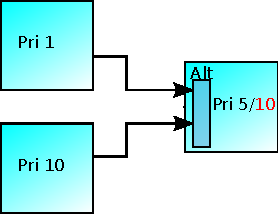
\includegraphics[scale=1.00]{images/alt-inheritance}
  \caption{Prioritetsnedarvning i \code{alternations.}}
  \label{fig:alt-inheritance}
  \end{center}
\end{figure}

\chapter{Eksempler}

\section{Hajer og fisk på Wator} Som eksempel på en DES simulation
har vi valgt at tage udgangspunkt i det scenarie som A. K. Dewdney
beskrev i artiklen \fixme[inline]{reference}. Artiklen beskriver den
fiktive planet Wator, der har form som en torus og er fuldstændig
dækket af vand. Verdenen er inddelt i felter som beskrevet på side
20 i \fixme[inline]{ref}. Disse felter kan være tomme, indeholde en
fisk eller en haj. Følgende karakteristika beskriver fisk og hajers
opførsel.


Fisk - bevæger sig og forplanter sig Lever af plankton, en ressource
som er uendelig. Hvis der er et ledigt tilstødende felt bevæger en
fisk sig til dette felt. Hvis der er flere ledige felter vælges et
tilfældigt. Hvis en fisk overlever 3 livscykler forplanter den sig.


Hajer - jager og forplanter sig Såfremt der er fisk i et eller flere
tilstødende felter flytter hajen sig herhen og spiser fisken. Hvis der
er flere tilstødende felter med fisk vælges et tilfældigt. Er der
ikke nogen fisk i nærheden bevæger en haj sig på samme måde som en
fisk. Hvis en haj ikke spiser i mere end 3 livscykler dør den. Hvis en
haj overlever 10 livscykler forplanter den sig.

For hvert tidsskridt vil alle fisk og hajer udføre en handling ud fra
ovenstående opførsel.

Til at initiere systemet skal der defineres en størrelse af verdenen,
samt hvor mange fisk og hajer der er til stede fra start. Disse fisk og
hajer placeres tilfældigt i verdenen.

Såfremt de initielle parametre understøtter en bæredygtig bestand
forventer vi at se bestanden af henholdsvis fisk og hajer oscillere
afhængigt af hinanden.

\section{Kunder i en bank} Et klassisk eksempel inden for \des

\section{Implementering}\label{sec:deadline-implementation}
Vi vil i dette afsnit beskrive hvilke ændringer og tilføjelser vi skal foretage i \pycsp, for at implementere RTP. Ændringerne vil tage udgangspunkt i de emner, vi har diskuteret i foregående afnit med fokus på de problemstillinger der skal tages højde for ved implementeringen af dem.  
\subsection{Overskredne deadlines}
%Planlægning i realtime kræver at man tager stilling til, hvordan  overskredne deadlines skal håndteres. Enten kan det opfattes som en egenskab for processen hvor dens deadline enten kan være overholdt eller ej, eller også kan en overskreden deadline resultere i en exception.

%Hvilken metode, der egner sig bedst til RTP, afhænger af hvilken deadline, der er tilknyttet processen. Er der tilknyttet en soft deadline til en proces, vil processen stadig tilføje værdi til systemet, selvom det overskrider dens deadline. Derfor kan det stadig være bedst for systemet at fuldføre processen til ende. I dette tilfælde  skal systemet blot markere at dens deadline er overskredet, og senere må programmøren så manuelt håndtere den overskredne deadline. 

%Hvis en proces har tilknyttet  en hard deadline, vil en overskredet deadline ikke tilføje værdi til systemet, og derfor kan det ikke betale sig for systemet at lade processen blive færdig. Processen skal derfor stoppes hurtigst muligt, så systemet i stedet kan udføre de processer hvis deadline endnu ikke er overskredet. For et system, hvor processerne har hard deadlines, vil det derfor være bedst, hvis en overskredet deadline resulterer i en exception, der med det samme stopper processen, og lader programmøren bestemme hvordan processen skal forholde sig til at deadlinen er overskredet.

%Vi har valgt, at der i vores system skal kaldes en exception, hvis en deadline overskrides. Dette er gjort ud fra en betragtning om, at systemet ikke kender konsekvensen af en overskredet deadline, men på processniveau har udvikleren tilføjet en deadline, og derfor må det være udviklerens ansvar at håndtere processen ved en overskridelse af deadline.  Hvis processen stadig kan bidrage med værdi, kan programmøren lade processen fortsætte sin kørsel. Alternativt kan processen lukkes korrekt ned. Ulempen ved at kalde en exception er, at processen stopper sin eksekvering i utide, hvilket kan give problemer, f.eks. hvis processen er tilknyttet en kanal og venter på at kommunikere.  Kanalerne holder i \pycsp styr på antallet af processer, der vil kommunikere, og hvis processen pludseligt forsvinder vil tilstandsvariablerne ikke være sat korrekt. Det er derfor vigtigt at processen korrekt fjerne sig selv fra kanalen i forbindelse med en exception.
Vi har i foregående afsnit argumenteret for, at alle overskredne deadlines bør resultere i en exception. Dette er oplagt at implementere i \sched en, så det checkes ved kontekstskift, om en deadline for den proces der skiftes fra, er overskredet, og i givet fald, kaster en exception. Vi ønsker dog at få kastet vores exceptions så hurtigt som muligt, for derved at gøre opmærksom på den overskredne deadline. Derfor checker vi yderligere for overskredne deadlines, når der kommunikeres på en kanal, og når der foretages et valg i en \code{alternation}. 
\fxnote{Mere i dette afsnit ville være rigtig rart}

\subsection{Ændringer i \sched en}
\phantomsection
\label{sec:sched-changes}
I \code{greenlets}-versionen af \sched en findes der som nævnt i \cref{sec:scheduler} tre lister af processer: \code{new}, \code{next} og \code{timers}. De tre lister er prioriteret således, at der først kigges på processer fra \code{timers}, dernæst fra \code{new} og til sidst kigges der i \code{Next}.

I RTP er det ikke hensigtsmæssigt at inddele processerne i disse tre  kategorier. Vi skal derimod have et miljø, der gnidningsløst tillader processer både med og uden deadlines, samt at de dynamisk kan ændres. Skemaplanlæggeren skal i forbindelse med processkift hurtigt kunne finde den næste proces, der skal udføres.

Vi har derfor valgt at fjerne  de tre lister og erstatte dem  med \code{has"_priority},  \code{no"_priority} og \code{timers}. \code{has"_priority} og  \code{no"_priority}  benyttes til aktive processer, der ønsker at blive udført, mens \code{timers} er en kopi af \des versionen. 

Det er vigtigt at bemærke ifht. processer der ligger i \code{timers}, at udvikleren ikke kan forvente at de bliver aktiveret på de eksakte tidspunkt han har defineret. Dette er kun muligt i \des versionen hvor vi kan kontrollere tiden. Den eneste garanti der gives, når vi arbejder med realtid, er at de tidligst aktiveres på det angivne tidspunkt. I \code{greenlets}-versionen  aktiveres først processer fra \code{timers} listen. Dette gøres fordi processer i denne version kun kommer på denne liste via \code{timeout}-guarden. En udvikler vil forvente  at processen venter i præcist det tidsrum man har angivet for så at fortsætte. For at emulere dette krav om kun at vente et præcist tidsrum foretrækkes derfor processer fra denne liste fremfor processer der bare ønsker at bliver kørt. I RTP antages det, at der findes en mængde processer, der skal gennemføres inden en deadline, hvorfor de må kæmpe om CPU-tid. En proces, der har ventet i \code{timers} listen skal derfor ikke nødvendigvis udføres med det samme, da det hele tiden bør være den proces med den højeste prioritet der skal udføres, uafhængigt af processerne i \code{timers} hoben. Processerne, der ikke længere skal vente på timeout, bliver derfor planlagt og udvalgt på lige fod med andre processer der er klar til at blive udført. 

Til at implementere \code{has"_priority} bruger vi også en hob, men da modulet \code{heapq} kun understøtter min-hobe kan vi ikke lave en klassisk prioritetshob, da den skal kunne udtrække processen med maksimal prioritet. Vi har dermed to muligheder, enten kan vi lave vores egen implementering af en maks-hob, eller også kan vi ændre vores prioriteter internt, så en lav værdi angiver en høj prioritet. Med en egen implementering har vi en  logisk opbygning af prioriteter, men vi får ikke fordelen ved den underliggende implementering  direkte i C, som man opnår ved brug af modulet heapq. Vælger vi at bruge dette, skal vi invertere prioritetsbegrebet, så det er den laveste prioritet, der udvælges først. Dette viser  sig dog ikke at være et problem  i vores tilfælde, da vi ønsker at benytte os af en EDF algoritme og derfor nemt kan opnå den ønskede effekt ved at bruge en proces' deadline som dens prioritet. Her vil en lav deadline betyde, at processen snart skal være færdig, hvilket resulterer i en høj prioritet.
Vi kan derfor blot benytte en proces' deadline som dens prioritet og benytte en min-hob. 

%Hvis man i en fremtidig version ønsker at udvide vores \sched , så en udvikler kan tilknytte bruger-prioriteter til proceserne, kan det f.eks implementeres ved efterfølgende at ændre \sched ens prioritet. Dette vil resultere i at processen bliver opprioriteret ifh. til andre processer.

\subsection{Preempting}

Som vi har beskrevet i \cref{sec:rtp-pycsp}, kan  man risikere, at en proces med lav prioritet proces og kørselstid\fxwarning{``med lav prioritet og kørselstid'' hvad betyder det?} kan blokere for en proces med høj prioritet. 
Her konkluderede vi at det er udviklerens opgave at processen afgiver kontrol, og derfor skal det være nemt at afgive kontrollen for processen. Til dette har vi lavet funktionen \code{Release()}, der minder om \code{Yield} for \code{co-rutiner}.

Implementeringen er meget simpel og er blot en wrapperfunktion, da den underliggende funktionalitet allerede eksisterer. Den aktive proces stopper og bliver genplanlagt til senere kørsel af \sched en. Dermed lægges processen på den relevante kø, og  \sched en får mulighed for at vælge en ny proces der skal udføres. Er der ikke kommet nye processer, vil det stadig være den originale proces, der vælges og kan fortsætte sin kørsel. Hvis der derimod er ankommet en eller flere nye processer i mellemtiden, som har højere prioritet, vil disse blive valgt i stedet.

Problemet ved denne tvungne procesafgivelse er, at det kan tage lang tid at lægge processerne i en min\_hob, som vil være spildt, hvis den alligevel med det samme fjernes fra køen. Man vil derfor nok i en senere version kunne optimere hastigheden af \code{Release()}.

\subsection{Udvidelse af \code{Process}}
Hver proces skal kunne tilknyttes en deadline, som er et tidsstempel, der angiver det tidspunkt, som udvikleren ønsker at processen skal være færdig inden. 
Desuden skal hver proces tilknyttes en prioritet. Denne prioritet bruges af \sched en til at udvælge hvilken proces der skal eksekveres. I EDF er prioriteten og deadline for en proces som  den samme, og prioriteten er derfor også et tidsstempel.

I forbindelse med prioritetsnedarvning kan en proces midlertidigt få ændret sin prioritet, hvilket vi diskuterer yderligere i \cref{sec:deadline-implementation-priorityinheritance}. For at kunne adskille prioriteten, der ikke altid er sat af udvikleren, og en deadline, der altid er sat af udvikleren, har vi  valgt at holde de to variable adskilt. 

Når en proces bliver udvalgt til at arve en prioritet gennem prioritetsnedarvning, skal \sched en  planlægge processen ifht. den nye prioritet.
Den nye prioritet er også et tidsstempel, og hvis ikke processen er færdig, inden denne prioritet er overskredet, vil en anden proces' deadline være overskredet. 
Vi kan derfor vælge at \code{RTP} skal kaste en  \code{deadlineException},  hvis  prioriteten overskrides. Ved at kaste en \code{deadlineException} i processer hvor prioriteten er overskredet, kan udvikleren se præcist hvilken proces, der var aktiv, og dermed se hvorfor den originale proces også kaster en \code{deadlineException}. 

\CRef{fig:producer-worker-consumer} viser et tidsdiagram for et generator/arbejder/forbruger-netværk bestående af tre processer B$_1$, B$_2$ og B$_3$. B$_3$ har den højeste prioritet, og B$_2$ arver denne prioritet. Hvis B$_2$ også kaster en \code{deadlineException} vil det tydeligt fremgå for udvikleren, at det er B$_2$ der bærer skylden for, at B$_1$'s deadline ikke blev overholdt.

En anden begrundelse for at lade en nedarvet prioritet medføre en \code{deadlineException} er hvis processerne er afhængige af hinanden. I \cref{fig:producer-worker-consumer}  nedarver  arbejderprocessen(B$_2$) og generatorprocessen (B$_1$) en  prioritet fra forbrugerprocessen (B$_3$). Hvis denne deadline ikke nås, er det data som arbejderprocessen bearbejder ikke længere relevant, og arbejderprocessen kan med fordel stoppe det irrelevante arbejde. I eksemplet ville arbejderprocessen (B$_2$) kunne stoppe sit arbejde til tiden $t = 5$ i modsætning til at fuldføre arbejdet, og stoppe i tiden $t = 6$.

\begin{figure}
 \begin{center}
  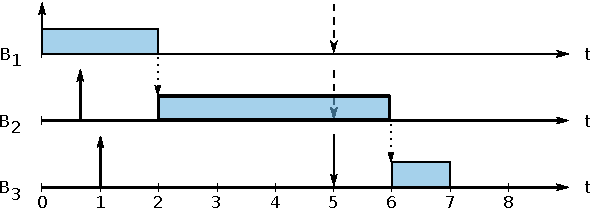
\includegraphics[scale=1.00]{images/producer-worker-consumer}
  \caption{Et generator/arbejder/forbruger -netværk. Kasserne repræsentere det tidsrum hvor processerne bliver bearbejdet. En pil op indikere hvornår processen er klar til at blive eksekveret. En pil ned indikere en deadline for processen. De stiplede pile i proces B$_1$ og B$_2$ til tiden t$=5$ viser en kunstig prioritet på baggrund af B$_3$'s deadline. Den lille stiplede pil mellem  B$_1$ og B$_2$ i t$=2$ og mellem B$_2$ og B$_3$ i t$=6$ viser kommunikation mellem processerne.}
  \label{fig:producer-worker-consumer}
  \end{center}
\end{figure}
\fxnote{Skriv på figurene hvem der er generator/arbejder/forbruger}
\begin{figure}
 \begin{center}
  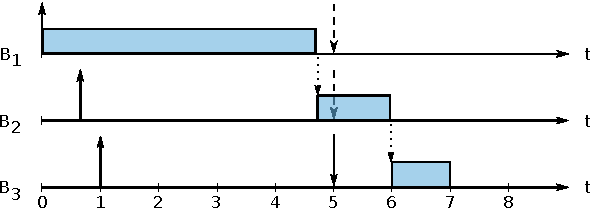
\includegraphics[scale=1.00]{images/producer-worker-consumer2}
  \caption{Samme netværk som i \autoref{fig:producer-worker-consumer}, men i dette tilfælde venter B$_2$  på data fra B$_1$ i hovedparten af tiden inden en deadline.}
  \label{fig:producer-worker-consumer2}
  \end{center}
\end{figure}


Der er dog ikke sikkert at en deadlineException i processer der har nedarvet en prioritet, er med til klarlægge hvilke processer der har brugt al tiden, og derfor bærer skylden for at en deadline ikke blev overholdt. \CRef{fig:producer-worker-consumer2} viser et eksempel på dette. Netværket er opsat som i \autoref{fig:producer-worker-consumer}, men i dette tilfælde bruger generatorprocessen (B$_1$) al tiden, og data bliver først sendt fra $B_1$ umiddelbart før en overskridelse af deadlinen. For en udvikler  vil det fremgå, som var det arbejderprocessen (B$_2$), der er ansvarlig for overskridelsen ligesom i \autoref{fig:producer-worker-consumer}, og ikke generatorprocessen $B_1$, som i dette eksempel brugte det meste af tiden. Dermed mister \code{deadlineException} sin troværdighed, og brugbarhed til at identificere hvor i netværket tiden bruges. 

Et andet problem ved at lade den aktive proces kaste en \code{deadlineException} er, at det vil pålægge udvikleren et væsentligt større arbejde med at håndtere disse exceptions. Såfremt vi implementerer det, kan enhver proces, der kan arve en prioritet via prioritetsnedarvning, kaste en exception. Det er ikke nødvendigvis klart gennemskueligt hvilke processer det vil være, hvorved udvikleren kan have svært ved at sikre ordentlig fejlhåndtering. Yderligere vil det medføre at excpetions kan kastes udenfor den kontekst de er relateret til, hvorved det kan være umuligt at håndtere dem korrekt.  

På baggrund af de opstillede fordele og ulemper, har vi valgt at kun processer med en eksplicit deadline, har mulighed for at kaste en \code{deadlineException}. Processer, der nedarver en prioritet, bliver planlagt i henhold til den højeste prioritet, de har, og vil altid  gøre arbejdet færdigt. En proces skal dermed kunne adskille sin egen deadline fra den prioritet, som den skal planlægges med, selv om de to værdier i en stor del af tiden vil være det samme.

En deadline er dermed en variabel der kun kan sættes af udvikleren og det er kun på baggrund af denne deadline at  processen skal kaste en \code{deadlineException}.

For at  \sched en kan udvælge processer introduceres prioritet, der som standard er det samme tal som deadlinen. For at kunne håndtere flere niveauer af prioritetsnedarvning,  gemmes prioriteten i en  liste kaldet \code{inherit\_priotity}. Denne liste af prioriteter  indeholder indledningsvis kun en prioritet som er deadlinen sat af udvikleren. Når andre processer  midlertidigt ønsker at ændre en proces' prioritet, tilføjes den til listen. Ved at bruge en liste i stedet for blot en variabel, har processen mulighed for at blive opprioriteret flere gange og derefter trinvist vende tilbage til de tidligere niveauer.

Når \sched en placerer processen i hhv. \code{has\_priority} og \code{no\_priority} hobene, bruges blot den mindste prioritet i listen af nedarvede prioriteter ihht. vores implementering af \sched en. Dette medfører, at når en proces efterfølgende  får ændret sin liste af prioriteter, skal processen genplanlægges for at sikre, at den placeres korrekt i min-hoben i \sched en. 

\subsection{Kanaler}
I \pycsp findes der kun kanaler af typen \code{Any-To-Any}, og derfor kan der altid  være et vilkårligt antal kanalender i hver ende af kanalen, der kan være klar til at kommunikere. Vi skal derfor foretage en ændring, så kommunikationen mellem kanalenderne altid foregår mellem de højst prioriterede processer. 

I greenletsversionen foregår udvælgelsen af kanalender til kommunikation ved hjælp af funktionen \code{match}, der udnytter at  hver kanal vedligeholder to lister af processer for hhv. de processer, der ønsker at sende, og modtage data på kanalen. Når en proces eks. ønsker at modtage data, tilføjer den sig selv til listen af processer, der ønsker at modtage, og prøver derefter i \code{match} funktionen at finde en proces, der vil sende data. Er der ingen processer, der venter på at sende data, venter processen på, at en proces melder sig klar til at sende data, ved at kalde \code{match}. Til hver vellykket kommunikation af data vil \code{match} altid blive kaldt to gange, hvor kun den sidste vil resultere i at kommunikationen lykkes.

Ideen bag funktionen \code{match} er enkel og  udnytter, at \code{greenlets}-versionen er enkelttrådet, så hver proces kan løbe listerne igennem, uden andre processer ændre på listernes tilstand.  Vi er kommet frem til, at  en simpel sortering af listerne ud fra processernes interne prioritet vil resultere i, at det altid er den højst prioriterede proces der indgår i kommunikationen. Den ændrede \code{match} kan ses i \cref{lst:match}, hvor det kun er linje 119 og 120 der er ændret.

\begin{lstlisting}[firstnumber=117 ,float=hbtp, label=lst:match, caption=Funktionen \code{match} der sorterer kanalrequests.]
def match(self):        
    if self.readqueue and self.writequeue:
        self.readqueue.sort(key=lambda channelReq:channelReq.process.internal_priority)
        self.writequeue.sort(key=lambda channelReq:channelReq.process.internal_priority)
        for w in self.writequeue:
            for r in self.readqueue:
                if w.offer(r):
                    return       
\end{lstlisting}

Funktionen \code{match} vil blive kaldt en gang for hver proces der ønsker at kommunikere, og derfor vil det kun være det sidste element i listen som ikke er sorteret korrekt ved hver kald af \code{match}. Desuden vil der altid i den ene liste maksimalt være på et element. Bemærk desuden at listerne er sorteret så værdien af den interne prioritet er stigende, og derfor er det processen med lavest værdi, der først bliver udvalgt til et match, i overensstemmelse med repræsentationen af prioriteter som nævnt i afsnittet ``Ændringer i \sched en'' %\vpageref{sec:sched-changes}.
på side \vpageref{sec:sched-changes}.
\fxerror{ret til vpageref}


\subsection{Prioritetsnedarvning}
\label{sec:deadline-implementation-priorityinheritance}
Prioritet i et RTP system skal ses i forhold til alle processers prioritet. En proces kan derfor ikke i sig selv have en absolut høj prioritet, men kun have høj prioritet ifht. de andre processers prioritet. Ved at give en høj prioritet til  en proces, vil dette dermed  indirekte sænke de andre processers prioritet, et fænomen vi vil kalde ``prioritetsdevaluering``.

For at minimere prioritetsdevaluering i forbindelse med prioritetsnedarvning, ønsker vi at minimere den tid en proces har en kunstigt høj prioritet, og at minimere antallet af processer, hvis prioritet øges. 

Som vi er kommet frem til i \cref{sec:rtp-pycsp-nedarvning}, skal  der foregå  prioritetsnedarvning i forbindelse med kommunikation, hvis der ikke findes nogle processer, der umiddelbart er klar til at kommunikere.  I \pycsp kan man umiddelbart evaluere, om der er processer klar til at kommunikere over en given kanal. Det skyldes, at processer der ønsker kommunikation befinder sig i listerne \code{readqueue} og \code{writequeue}. Hvis ingen processer ønsker at kommunikere, kan man dog ikke finde de processer som potentielt kan indgå i kommunikation.
Vi må derfor udvide kanalerne i RTP versionen med to lister, \code{readerprocesses} og \code{writerprocesses}, der består af de processer, der potentielt kan sende og modtage data over kanalen. Vi håndterer vedligeholdelsen af disse lister, ved at hver proces ved opstart tilføjer sig selv til de kanaler, den har mulighed for at kommunikere over. Et oplagt sted at implementere denne funktionalitet er i processens  \code{\_\_init\_\_}  funktion, da alle kanalender som denne proces potentielt kan kommunikere over, findes som argument til  \code{\_\_init\_\_} funktionen. \CRef{lst:process-init} viser udvidelsen af funktionen, hvor argumenterne gennemløbes, mens der ledes efter kanaler, som processen skal registreres i.

\begin{lstlisting}[firstnumber=29 ,float=hbtp, label=lst:process-init, caption=Uddrag af \code{Process}' \code{\_\_init\_\_}funktion]
for arg in args:
    if isinstance(arg, pycsp.greenlets.channelend.ChannelEndRead):
        arg.channel._addReaderProcess(self)
    if isinstance(arg, pycsp.greenlets.channelend.ChannelEndWrite):
        arg.channel._addWriterProcess(self)  
\end{lstlisting}

Kanaler kender nu  både de processer, der på et specifikt tidspunkt ønsker at kommunikere vha. listerne \code{readqueue} og \code{writequeue}, og de processer, der potentielt vil kunne kommunikere vha. listerne \code{readerprocesses} og \code{writerprocesses}. Processer der ønsker at kommunikere kan, som normalt umiddelbart evaluere om det er muligt; såfremt det ikke er muligt, kan den nu evaluere hvilke processers prioritet den kan øge, for at bringe dem i en tilstand hvor de kan indgå i den ønskede kommunikation. 

Funktionaliteten til prioritetsnedarvning skal implementeres i de to interne kommunikationfunktioner  \code{\_read} og \code{\_write}. Fordelen ved at placere prioritetsnedarvning i disse to funktioner er, at de bruges af processerne både i forbindelse med normal blokerende kommunikation og i forbindelse med kommunikation i \code{alternation}. Vi har udvidet funktionerne med følgende liste af begivenheder:
\begin{itemize}
\tightlist
	\item Undersøg om processen opfylder kriterierne for at starte en prioritetsnedarvning.
	\item Forhøj prioriteterne for de potentielle processer i enten \code{readerprocesses} eller \code{writer\-processes}.
	\item Umiddelbart efter kommunikationen nedprioriteres de processer, man midlertidigt har øget prioriteterne på.
\end{itemize}

Som beskrevet er det vigtigt, at vi igennem hele designet forsøger at begrænse mængden af prioritetsnedarvningen, og derfor har vi tilføjet en række egenskaber, der skal være indfriet, før prioritetsnedarvning forsøges. Disse er: processen skal have en prioritet, enten direkte eller efter en nedarvning; kanalen må ikke være klar til kommunikation, hvilket vil sige, at hvis processen ønsker at skrive, må der ikke findes en proces, der er klar til at modtage data; endeligt skal processen ikke have overskredet sin egen deadline, da denne til slut blot vil kaste en exception, og hele prioritetsnedarvningen vil være irrelevant.

Selve prioritetsforhøjelsen og den senere nedprioritering er simpel, da processen blot sender sin prioritet til alle processerne i den relevante liste dvs. \code{writerprocesses} for  \code{\_read} funktionen og vice versa. Hvis en proces modtager en lavere prioritet end dens egen prioritet, ses der bort fra hhv. op- og nedjusteringen, så en prioritetsnedarvning ikke resulterer i en forringelse af prioritet. 

\subsection{\code{Alternation}}

Som nævnt i afsnit \cref{misc:kanal-prioritet} har vi behov for at kunne tilknytte en prioritet til en kanal for at kunne håndtere udvælgelse i \code{alternations}. Vi har allerede prioriteter for processer og ønsker, at kanalernes prioritet skal defineres på baggrund af hvilke processer, der er tilknyttet kanalen. Vi skal kunne håndtere både input- og output-guards og ønsker seperate prioriteter for disse. Vi tilknytter derfor to prioriteter til hver kanal. De to prioriteter er sat som  de højst prioriterede processer, der er klar til at hhv. modtage og sende data. En kanals prioritet er derfor ikke fast som for processerne, hvor de får sat en prioritet (der dog kan ændres med prioritetsnedarvning), men nærmere en emuleret prioritet, som ændre sig baseret på alle processernes tilstand. 

Til at implementere de to prioriteter introduceres  to hjælpefunktioner, der løber hhv. \code{readqueue} og \code{writequeue} igennem og  finder den højst prioriterede proces, der er villig til hhv. at sende og modtage data. Når  \code{alternation} ønsker at finde prioriteten for en kanal, kigger den på om kanalen i \code{alternation} er tilknyttet en output- eller inputguard og finder den korrekte prioritet.


\section{Evaluering}
\subsection{Test af Korrekthed}
Vi har som i \des løbende skrevet test før vi implementerede hver ny funktion i \code{RTP}-versionen.  Tabellen herunder viser testresultaterne for de test der er lavet specifikt for \code{RTP}-versionen.
\begin{longtable}{lr}
   	\toprule
    \mc{Test} & \mc{Resultat} \\
    \midrule
    \endfirsthead 
    \toprule
    \mc{Test} & \mc{Resultat} \\
    \midrule
    \endhead % slut efterfølgende headere
    \bottomrule
    \multicolumn{2}{r}{\textit{fortsættes}}
    \endfoot % slut footer
    \bottomrule
    \endlastfoot % slut sidste footer
test\_Alternation  & ok\\
test\_AlternationChoiseReader  & ok \\
test\_AlternationChoiseWriter  & ok \\
test\_AlternationExecuteReadDeadline  & ok\\
test\_AlternationExecuteSkipDeadline  & ok\\
test\_AlternationExecuteTimeoutDeadline  & ok \\
test\_AlternationExecuteWriteDeadline  & ok \\
test\_Alternationchoise1Deadline  & ok \\
test\_Alternationchoise2Deadline  & ok \\
test\_ChoisemultipleReader  & ok \\
test\_ChoisemultipleReader2  & ok \\
test\_ChoisemultipleWriter  & ok\\
test\_PoisonAndDeadline1  & ok\\
test\_PoisonAndDeadline2  & ok\\
test\_Reader\_Inheritance  & ok\\
test\_RetireAndDeadline  & ok\\
test\_Writer\_Inheritance  & ok\\
test\_channelpriority\_from\_low\_deadline  & ok\\
test\_channelpriority\_from\_low\_deadline2  & ok\\
test\_channelpriority\_from\_no\_deadline  & ok\\
test\_channelpriority\_from\_no\_deadline2  & ok\\
test\_readDeadline  &ok\\
test\_writeDeadline  & ok\\
test\_xreset\_inheritance  & ok\\
test\_xreset\_inheritance\_from\_two\_step  & FAIL\\
\end{longtable}


 Alle test med en undtagelse fungerer korrekt. Testen der fejler hedder test"_xreset"_inheritance"_from"_two"_step, og viser en situation hvor den samme proces får løftets sin prioritet to gange i træk, først med en høj prioritet, og efterfølgende med en mellemprioritet. Efterfølgende skal processen sænke sin prioritet, først til  mellemprioriteten og tilslut til sin originale prioritet. Her viser det sig vi har lavet en fejl i implementeringen, således at prioriteten ikke bliver nedsat til mellemprioriteten. \CRef{fig:priority-inheritance} viser prioriteten mens processen bliver op og nedprioriteret. Tiden har ikke tilladt os at løse problemet, men  kan løses ved at kræve at, når en proces opprioriteres gemmes hvilken proces der står bag, så når en proces ønsker at fjerne sin opprioritering fra andre processer er det kun sin egen  prioritet den fjerner.  
 
  
\begin{figure}
 \begin{center}
  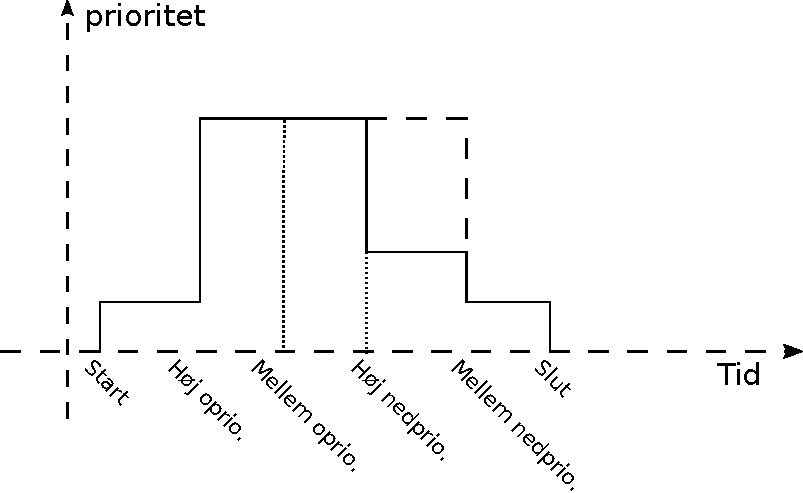
\includegraphics[scale=1]{images/priority-inheritance}
	\caption{Figuren viser hhv. forventet og faktisk prioritetsarvning. Der hvor den faktiske og forventede opførsel adskiller sig er forventet den fuldt optrukne streg, mens den stiplede streg er den faktiske opførsel.}
	\label{fig:priority-inheritance}
\end{center}
\end{figure}
  

\subsection{Slagterieksempel}

Først vil vi sammenligne de to udviklede versioner, for at se på deres fordele og ulemper, og til slut vi i dette afsnit sammenholde de to versioner, med et  eksempel der er implementeret i RTP-versionen.

Helt generelt opnår man når man ved brug af \pycsp et netværk, der nemt kan udvides hvis de fysiske rammer for slagteriet ændre sig. Viser det sig f.eks at kameraet holder den samlede produktivitet af netværket tilbage kan, slagteriet tilføjet endnu et kamera, og nemt udvide procesnetværket med endnu en kameraproces, som kan arbejde samtidigt med det første kamera. 

Forskellen i kode mellem \code{greenlets} og \code{proces}-versionen består af en linje, som indikerer hvilken version \pycsp skal bruge. En kørsel mellem de to versioner giver dog forskelligt resultat, som vist i \cref{tab:deadline-runs}. Dermed har valget af version betydning for både andelen af griseobjekter, der kan nå at blive bearbejdet, og hvor lang tid det tager i køre testen. Dette skyldes at testen køres på en multikerne CPU hvor \code{proces}-versionen dermed har mulighed for at køre parallelt. \code{Greenelts}-versionen derimod er begrænset til kørsel af en proces hvorfor der er flere grise der ikke når at blive bearbejdet inden for sin deadline.

\begin{table}[htbp]
	\centering
	\begin{tabular}{lrr}
       	\toprule
        \mc{Version} & \mc{Succesrate (\%)} & \mc{Tidsforbrug (s)} \\
        \midrule
        Greenlets & 42 & 16,5\\
        Processes & 71 & 10,3\\
        \bottomrule
    \end{tabular}
	\caption[]{Gennemførslen af simulation hvor 100 grise bliver sendt igennem procesnetværket. }\\
	\label{tab:deadline-runs}
\end{table}

Forskellen på kørselstiderne skyldes at detektoren venter på at aflevere griseobjektet til kameraet, og først når objektet er afleveret venter detektoren et normalfordelt tidsrum. Om dette er en urealistisk opførsel vil kræve mere domæneviden. Kan detektoren f.eks styre transportbåndet der fører grisene hen til detektoren er det en rimelig antagelse, mens det er urealistisk hvis båndet kører uafhængigt at detektoren.

I \code{procees}-versionen findes der fire processer og dermed kan der bearbejdes fire griseobjekter samtidigt. Dette sikre at det er de fire  griseobjekter nærmest robotten der arbejdes på, men samtidigt betyder det at man maksimalt kan arbejde på fire grise samtidigt. Ved at øge antallet af griseobjekter man kan arbejde på, vil man få mere tid per gris til at foretage de nødvendige beregninger. Man kan derfor vælge at tilføje flere konverterings og analyseprocesser, da disse ikke er bundet op på specialiseret hardware, og på den måde øge antallet af processer der kan arbejde samtidigt. Dette vil dog øge antallet af processer der må kæmper mod hinanden for CPU-tid, og griseobjekterne vil desuden skulle kæmpe mod hinanden for at komme igennem netværket uden hensyn til hvilken gris der er nærmest robotten. Man risikere dermed en starvation situation hvor griseobjekter svarende til  grise længere tilbage på transportbåndet overhaler griseobjekter længere fremme på transportbåndet.

\code{RTP}-udvidelsen bygger på \code{greenlets}-versionen, og vil derfor have de samme begrænsninger som denne, som diskuteret i implementeringen i afsnit \cref{sec:deadline-exampel-implementation}. Der er dog også en række fordele som vi vil komme ind på her.

Ved implementering af slagterieksemplet i \code{RTP}-versionen, slipper de enkelte processer for at holde styr på tiden, og vurdere om den enkelte gris deadline er overskredet. Når de modtager en gris sætter de deres egen deadline til grisens via funktionen \code{Set\_deadline}.  Hver proces skal i modsætningen til \code{greenlets}-versionen, kunne håndtere at modtage en \code{DeadlineException}, som de i dette eksempel blot kan håndteres ved at smide den nuværende griseobjekt væk. Det kan de gøre, da robotten på dette tidspunkt tager en beslutning uden specialviden om grisen, og griseobjektet er derfor ikke længere er relevant. I stedet kan processen  gå i gang med modtage et nyt griseobjekt.

I \code{greenlets}-versionen kom vi ind på at processerne frivilligt skal afgive kontrollen, før robotten kan foretage udskæringen, men at der ikke findes en metode til midlertidigt at afgive kontrollen. Med \code{RTP}-versionen og funktionen \code{Release} har alle processer mulighed for at afgive kontrollen så robotten rettidigt kan foretage selve udskæringen. Hermed skal vi ikke introducere en delt datastruktur.
  
selvom det var nødvendigt at basere RTP på  \code{greenlets}-versionen, medfører det at  kun en proces kan være aktiv på samme tid. Dermed kan vi kun udnytte en processor, som  passer dårligt sammen med denne applikation, som det ses af \cref{tab:deadline-runs}.  Vi kan dog til dels afhjælpe dette problem ved at udnytte at der i \code{greenlets}-versionen, findes en \code{IO}-dekorering. Denne dekorering placerer en funktion i en separat tråd, så flere funktioner kan køre samtidigt. Man skal her dog være opmærksom på at GIL'en stadig forhindre parallel udførsel. Eventuel parallel udførsel vil derfor kræve at koden i IO dekoreringen, kalder eksterne moduler som diskuteret i \cref{chap:csp}. Denne mulighed for parallel bearbejdning af flere processer vil dog  som i \code{processes}-versionen resultere i at processerne vil kæmpe mod hinanden om CPU-resurser. \code{RTP}-versionen har dog den store fordel at vi sikrer vi i modsætning til \code{proces}-versionen ikke risikere at griseobjekterne overhaler hinanden, men at netværket hele tiden har fokus på først at videresende griseobejektet nærmest robotten. \CRef{fig:pig-network3} viser hvordan netværket kan se ud med flere konverterings og analyse processer. 

\begin{figure}
 \begin{center}
  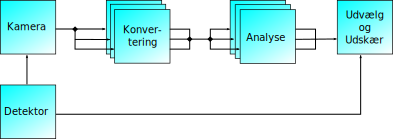
\includegraphics[scale=1]{images/pig-network3}
	\caption{Procesnetværk med flere konverteringsprocesser, og analyseprocesser}
	\label{fig:pig-network3}
\end{center}
\end{figure}

\section{Fremtidigt arbejde}\label{sec:deadlineFuture}
Vi har i dette kapitel opstillet en basal model for en RTP-implementering i \pycsp. Implementeringen er foretaget med henblik på blot at vise muligheden for en sådan model, og der er flere udviddelser som vi mener vil kunne forbedre modellen såfremt de kan implementeres. Vi vil i dette afsnit gennemgå nogle forbedringer som vi mener er interessante, men som ikke er inddraget i den basale implementering. 

\subsubsection{Evaluering af effektivitet}
Vi har med eksempler og test vist, at den implementerede løsning fungerer teoretisk korrekt. Vi har dog ingen reelle målinger af, hvor meget tid vi bruger på at evaluere hvilken proces der skal aktiveres, samt opretholde de metadata der skal til for at foretage denne vurdering. En grundig analyse af tidsforbruget i de administrative dele af vores implementering ville derfor være interessant at udføre, så man bl.a. kan udlede generelle retningslinier for, hvor ofte det vurderes hvilken proces der skal køre og hvor beregningstung hver proces bør være for at opnå den bedste ydelse. 

\subsubsection{Estimater for udførselstid}
Den primære begrænsning i vores løsning er manglen på at kunne evaluere hvor lang tid en proces eller dele af en proces tager at udføre. Hvis vi kunne udvikle en løsning der kunne foretage estimater af processers udførselstid ville vi kunne vælge en anden udvælgelsesalgoritme, som f.eks LL frem for EDF. Derved ville udvælgelsen af hvilken proces der skal aktiveres blive mere præcis. Ligeledes vil muligheden for at vurdere hvor langt en proces er nået i sin udførsel også være meget brugbart i forbindelse med prioritetsnedarvning. I vores implementering nedarver vi prioritet til alle processer som har mulighed for at opfylde en afhængighed. Såfremt vi kan vurdere hvilken proces der er tættest på at kunne opfylde afhængigheden, kan vi nøjes med at nedarve prioriteten til denne proces. Dette vil afhjælpe problemet med prioritetsdevaluering som nævnt i ``Ændring af prioritet'' i afsnit \ref{sec:aendring-af-prioritet}\vpageref{sec:aendring-af-prioritet}.

\subsubsection{Håndtering af forskellige typer deadlines}
I den nuværende løsning håndterer vi alle deadlines ens. Det er der fordele og ulemper ved, hvor en fordel er, at udvikleren får maksimal kontrol over hvad der skal ske såfremt en given deadline overskrides. Vi håndterer overskridelser af deadlines ved at kaste en exception når det sker. Dette er måske ikke altid ønskværdigt hvis det er en soft deadline der overskrides, da processen derved afbrydes. Det kunne tænkes at der er tilfælde hvor det er mere hensigtsmæssigt at udføre processen helt, og først her give besked om at den ikke nåede sin deadline.

%\fxerror*{Skal dette med}{I en fremtidig version ville man kunne udvide muligheden med en hybridversion, der skulle kunne håndtere processer med soft deadlines, der skal markeres, og kalde exceptions ved processer med hard deadline. Processen kunne f.eks have tilknyttet dens type af deadline. Systemet kan så reagere passende efter typen af deadlines, så soft deadlines blev færdigbehandlet, mens hard deadlines resulterede i en exception.}


\subsubsection{Udviklerbestemte prioriteter}
På nuværende tidspunkt har alle processerne den samme prioritet inden de planlægges, og deres prioritet afhænger udelukkende af deres deadline. Det kunne være interessant at undersøge om man kan bruge en anden skemaplanlægningsalgoritme, der kan håndtere at processerne har forskellige prioriteter inden de blev planlagt.

Hvis muligheden  for at differentiere processerne blev implementeret, kunne det være spændene hvis man kunne udvide \sched, så udvikleren kunne angive et kritisk sæt af processer, for hvilke det kunne garanteres at de ikke ville overskrider deres deadline. 

%\subsubsection{Implementering i andre \pycsp versioner}
%Det kunne være interessant at undersøge mulighederne for for at lave en implementering af RTP i andre versioner af \pycsp. Dette vil åbne op for de muligheder der er tilknyttet de forskellige implementeringer, hvilket vil gøre RTP mere praktisk anvendelig. Specielt er muligheden for brug af flere processorer med enten threads\footnote{Ved brug af eksterne moduler}- eller process-versionen. Dette vil dog, som tidligere nævnt, kræve at skemaplanlægningen flyttes til operativsystems skemaplanlægger og bliver derved 


%Test af effektivitet

%Estimater for kørselstid for processer

%Evaluering af hvor langt en proces er fra at være færdig

%Implemementering i process-version
\fxnote{Udvide kanaler til at være alternations med timeouts}

%\begingroup
%\setsecnumdepth{part} 
\chapter{Konklusion} 
\label{chap:konklusion}

Vores mål med dette speciale, var at undersøge muligheden for at lave en udvidelse af \pycsp, der muliggør brugen af tid direkte i sproget. Der findes allerede et massivt teoretisk arbejde indenfor området, men ingen praktisk anvendelig implementeringer, så vores fokus har været på at det skulle være praktisk anvendeligt. Dette afspejles ved at vi har valgt at benytte eksempler som omdrejningspunkt for vores analyser af de tre anvendelsesområder. 

De tre anvendelsesområder vi identificerede i introduktionen var diskret simulering, realtids-planlægning og interaktiv tid. 

Indenfor diskret simulering har vi udviklet en løsning, der er let at anvende, og som eliminerer kravet om en delt datastruktur for at administrere tid i \pycsp. Løsningen kræver væsentligt mindre kode til at administrere tiden, end en tilsvarende løsning lavet i ren \pycsp.  




Tidsmodeller/anvendelsesområder


Praktisk anvendelig implementering


nuværende tilstand for anvendelsesområderne

DES



RTP



IP


%\endgroup 


